\section{Implementation}
\begin{frame}{Overview}
    \begin{itemize}
        \item The implementation of the compiler is differentiate into four different stages:
        \begin{enumerate}
            \item Lexical and Syntactic Analysis
            \item Semantic Analysis
            \item Code Generation
            \item Optimizations
        \end{enumerate}
        \item The process is managed by a static compiler class.
        \item It parses the command line parameters, handles the input and output of files, and calls the different stages.
    \end{itemize}    
    \begin{figure}[htp]
        \centering     
        \lstinputlisting[style=bashstyle]{../figures/code/slides/cli_example.bash}
        \caption{A command line interface example.}
    \end{figure}
\end{frame}

\begin{frame}{Symbols and Symbol Table}
    \begin{minipage}{.45\textwidth}
        \begin{itemize}
            \item 
        \end{itemize}    
    \end{minipage}
    \begin{minipage}{.45\textwidth}
        \centering
        \begin{figure}[htp]
            \centering
            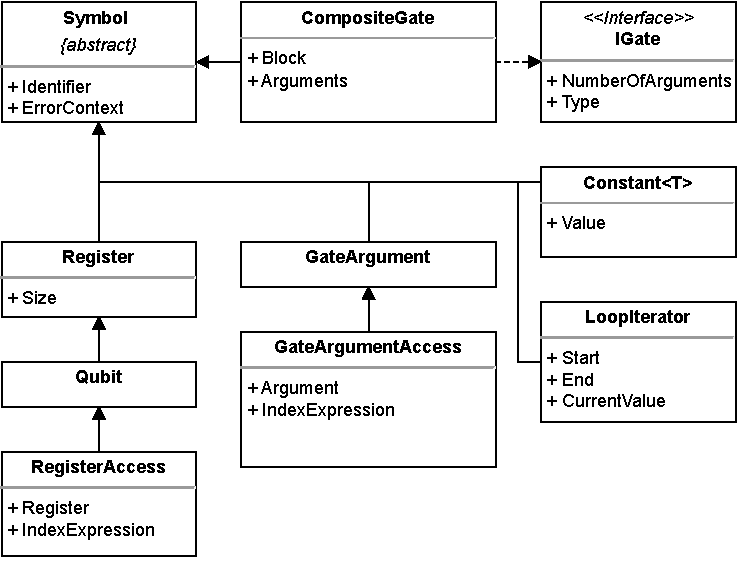
\includegraphics[width=.95\textwidth]{../figures/drawio/slides/uml_symbols.pdf}
            \caption{A diagram showing the hierarchy of symbol classes.}
            % \label{fig:implementation_uml_errors}
        \end{figure}
    \end{minipage}
\end{frame}

\subsection{Lexical and Syntactic Analysis}
\begin{frame}{Code Generation}
    \begin{itemize}
        \item 
    \end{itemize}
\end{frame}

\subsection{Semantic Analysis}
\begin{frame}{Code Generation}
    \begin{itemize}
        \item 
    \end{itemize}
\end{frame}

\subsection{Code Generation}
\begin{frame}{Code Generation}
    \begin{itemize}
        \item 
    \end{itemize}
\end{frame}

\subsection{Optimization}
\begin{frame}{Optimization}
    \dots
\end{frame}
